\documentclass{article}
\usepackage[utf8]{inputenc}
\usepackage{geometry}
\usepackage{nicefrac}
\usepackage{gensymb}
\usepackage[nowarnings]{xcookybooky}
\usepackage{imakeidx}
\usepackage{float}


\usepackage{hyperref} % this must be the last package that is imported!

\newcommand{\faren}{\degree F }
\renewcommand{\step} % fixing the error with xcookybooky somehow https://tex.stackexchange.com/questions/481698/missing-endcsname-in-package-xcookybooky-texlive
{%
 \stepcounter{step}%shouldn't be in the argument of lettrine
    \lettrine
    [%
        lines=2,
        lhang=0,          % space into margin, value between 0 and 1
        loversize=0.15,   % enlarges the height of the capital
        slope=0em,
        findent=1em,      % gap between capital and intended text
        nindent=0em       % shifts all intended lines, begining with the second line
    ]{\thestep}{}%
}
\geometry{
 letterpaper,
 left=1in,
 top=1in,
 }

\title{Recipes Not easy to print}
\author{Gaby Gerlach}
\date{\today}
\makeindex[intoc]

\begin{document}
\maketitle
\tableofcontents

\newpage
\section{Desert}
\begin{recipe}[source=Claire Saffitz]{Pecan Brittle Oatmeal Cookies}

\ingredients[15]{%
& \textbf{Pecan Brittle}\\
\unit[142]{g} & Coarsely chopped pecans \\
\unit[150]{g} & granulated sugar\\
\unit[57]{g} & unsalted butter \\
\unit[1/2]{tsp} & baking soda\\
\unit[1/2]{tsp} & kosher salt\\
& \textbf{Cookies}\\
\unit[2]{sticks} & unsalted butter, cut into tbsp\\
\unit[173]{g} & all-purpose flour\\
\unit[2]{tsp} & kosher salt\\
\unit[1]{tsp} & baking soda \\
\unit[200]{g} & old-fashioned rolled oats\\
\unit[150]{g} & dark brown sugar\\
\unit[100]{g} & granulated sugar\\
\unit[2]{large} & eggs (cold from the fridge)\\
\unit[1]{tbsp} & vanilla extract\\
}

\preparation{% 
\\
\textit{Make the Pecan Brittle}
\step Preheat oven to 350 \faren. Coarsely chop the pecans and bake until fragrant 8-10 minutes. Do not burn nuts!
\step Combine salt and baking soda in a small container set near stove. Place silicon baking mat on baking sheet, set aside.
\step Combine sugar and butter in sauce pan over medium heat with ~2 tbsp of water. Stir until melted than switch to swirling the pan (this prevents crystal formation). 
\step Boil until the sugar/caramel reaches a deep golden. Turn off the heat and working quickly stir in the pecans. Finally add the  baking soda/salt mixture and stir until combined.
\step Pour the mixture onto the baking mat and flatten to a single layer while warm. Set aside too cool.
\step Once cool and solid break it into large chunks using your hands and then cut so the largest pieces are about the size of a pea (it doesn't have to be neat). Set aside.
\\
\textit{Make the batter}
\step Make brown butter from ONE of the sticks of butter (you are only browning half of the butter)
\step Pour the browned butter into the bowl of your stand mixer with the other stick of butter. This now needs to cool to room temperature.
\step Put the flour, baking soda, half of the oats, and half of the pecan brittle into the food processor and pulse until you have formed a flour. 
\step Add the brown and white sugar to the mixer and combine. Add the cold eggs one at a time and combine. Add the flour mixture and carefully combine.
\step Scoop 2 once (1/4 cup) blobs onto a baking sheet and refrigerate for 24 hours.
\step Preheat oven to 350 \faren. Place 6 dough balls on a lined baking sheet (they spread) and bake for 16-20 minutes rotating once after 12 minutes. 
}

\hint{
You can freeze the dough balls after they have been in the fridge for a delicious single cookie whenever you feel like turning on the oven!
}
\end{recipe}

\begin{recipe}[source = Laura Howerton]{Ginger Cookies}
\ingredients[15]{
\unit[4]{cups} & All-purpose flour \\
\unit[2]{sticks} & unsalted butter \\
\unit[2]{tsp} & baking soda \\
\unit[4]{tbsp} & ground ginger \\
\unit[1]{tbsp} & ground clove \\
\unit[1]{tbsp} & nutmeg \\
\unit[2]{tbsp} & cinnamon \\
2 & eggs\\
\unit[1/2]{cup} & molasses \\
\unit[1]{cup} & granulated sugar \\
\unit[1]{cup} & brown sugar\\
}

\preparation{
\newline
\step Pre-heat oven to 350 \faren.
\step In a medium bowl stir together flour, ginger, baking soda, cinnamon, cloves, and salt; set aside.
\step In a large mixing bowl beat butter for 30 seconds, add the brown and white sugar, beat until combined. Beat in eggs and molasses until combined.
\step Add the dry ingredients to the wet ingredients.
\step Shape dough into 1-inch balls, place on cookie sheet and bake for 8 to 9 minutes until just done with the tops puffed. Cool on a wire rack.
}
\end{recipe}
\newpage

\section{Yeast-y baking} \begin{recipe}[source=Bob's Red Mill Bakery]{Rye
		Bread}

\ingredients[15]{ \unit[2 1/4]{tsp} & active dry yeast \\ \unit[1 1/4]{cups}
									& warm water \\ \unit[1 1/2]{tsp} &
		molasses \\ \unit[1]{tbsp} & Oil \\ \unit[1 3/4]{cups} & bread flour
		\\ \unit[1]{cup} & dark rye flour \\ \unit[2]{tbsp} & vital wheat
		gluten \\ \unit[1]{tbsp} & caraway seeds \\ \unit[1 1/2]{tsp} & salt
\\ }

\preparation{ \newline \step Sprinkle yeast over water and molasses in a
		large mixing bowl and let sit for 5 minutes. Add remaining
		ingredients and mix until dough pulls away from the sides of the
		bowl. Turn dough onto a lightly counter and knead for about 10
		minutes, or until you can stretch a small portion of the dough into
		a thin membrane. I was not able to knead enough with an electric
		mixer.  \step place dough in a clean oiled bowl. Cover and allow to
		rise until doubled. Punch down dough, cover and let rise another 15
		minutes. Preheat oven to 350 \faren and lightly oil a loaf pan.
		\step place dough on a lightly floured counter, shape into a loaf
		and place in prepared pan. cover and let rise for about 1 hour or
		until the dough crowns above the pan and gives with a gentle press
		of the fingers, leaving a faint indentation.  \step Bake for 30
		minutes or until golden-brown and hollow sounding when tapped. Cool
		on a wire rack.  } \end{recipe}
\newpage
\begin{recipe}[source=Bon Appetit]{Classic Focaccia Bread} 
		\begin{figure}[h!]
		\centering
		\includegraphics[width=0.5\textwidth]{photos/foccacia.jpeg}
\end{figure} 
		\ingredients[9]{ \unit[850]{g} & Bread flour \\ \unit[2
		1/4]{tsp} & active dry yeast \\ Pinch & sugar \\ \unit[2]{tbsp} &
Diamond Crystal or 1 tbsp Kosher salt \\ \unit[5]{tbsp} & extra-virgin olive
oil, divided \\ & flaky sea salt \\ & any other toppings\\ }

	\preparation{ \newline \step Combine flour and 2 1/2 cups of
			room-temperature water in the bowl of a stand mixer fitted with
			the dough hook. Mix on low speed unitl a shaggy dough forms.
			Cover and let sit while you prepare the yeast.  \step Stir
			yeast, sugar and 1/2 cup warm water with a fork in a small bowl.
			Let sit until the yeast is foamy.
			\step Pour yeast mixture into stand mixer bowl and mix on low
			speed until dough absorbs all additional water. BE CAREFUL IT
			WILL SPLASH if you don't go slow. Add kosher salt and mix until
			the dough is extremely elastic and very sticky, about 5 minutes
			(the dough will look like a batter).
			\step Pour 3 tbsp oil into a large bowl and swirl to coat sides.
			Scrape in dough cover and place in a warm spot until it has
			doubled in volume.
			\step Drizzle 2 tbsp oil over a 18x 13 sheep pan and rub all
	over bottom and sides. Using a large spatula, fold dough inside bowl a
	couple of times to deflate, then scrape onto prepared baking sheet.
	Using oiled hands, lift up dough and fold over onto itself in half, then
	rotate baking sheet and fold in half again. Cover dough with a piece of
	well-oiled plastic and let rest for 10 minutes to let gluten relax. 
			\step With oiled hands, gently stretch the dough across the baking
			sheet in an even layer. Working all the way to edges and into
			corners. If dough starts to spring back, let sit for 5-10 minutes
			and start again. Cover with oiled plastic and chill at least 8
			hours and up to 24.
			\step Preheat oven to 450 \faren with a rack in the center, let
			dough sit out at room temperature for 45-65 minutes until doubled
			in height.
			\step Remove plastic and drizzle dough generously with more oil.
			Oil hands and press fingertips firmly into dough pushing all the
			way to the bottom of the pan to dimple all over. Sprinkle
			generously with sea salt and any other toppings.
			\step Bake until surface is deep golden brown, 25-35 minutes, let
	cool in pan 10 minutes. Slide a spatula underneath to loosen and transfer
	to a wire rack.  }
\end{recipe}
\newpage
\begin{recipe}[source = Sally's Baking Addiction]{Homemade Bagels}

		
		\ingredients[8]{
		\unit[1 1/2]{cups} & warm water \\
		\unit[1 3/4]{tsp}& active dry yeast \\
		\unit[500]{g} & bread flour \\
		\unit[1]{tbsp} & packed brown sugar \\
		\unit[2]{tsp} & salt \\
		& 1 egg white \\
		\unit[1/4]{cup} & honey \\
						& any toppings \\
		}
	
		\preparation{
		\step Whisk the warm water and yeast together in the bowl of your stand mixer fitted with a dough hook attachment. Cover and allow to sit for 5 minutes.
		\step Add the flour, brown sugar, and salt. Beat to combine then kneed with the dough hook until it is quite stretchy. Cover the dough and allow to rise until doubled in size 60-90 minutes.
		\step Fill a wide pot with water and the honey and bring to a rapid boil. Pre-heat the oven to 425 \faren.
		\step Shape the bagels. Punch down the dough and divide into 8 equal pieces. Shape each piece into a ball and then press your index finger though.
		\step Make an egg wash by combining the egg white and 1 tbsp water.Drop the bagels in the boiling water 2-4 at a time and cook for 1 minute on each side.
		\step Using a brush coat the egg wash on the top and sides of each bagel. At this time you can add any toppings to the bagels. Bake for 20-25 minutes rotating halfway through the bagels should be a dark golden brown. Allow to cool and serve as desired. 
		}
		\begin{figure}[h]
				\begin{subfigure}{.5\textwidth}
						  \centering
						    % include first image
						    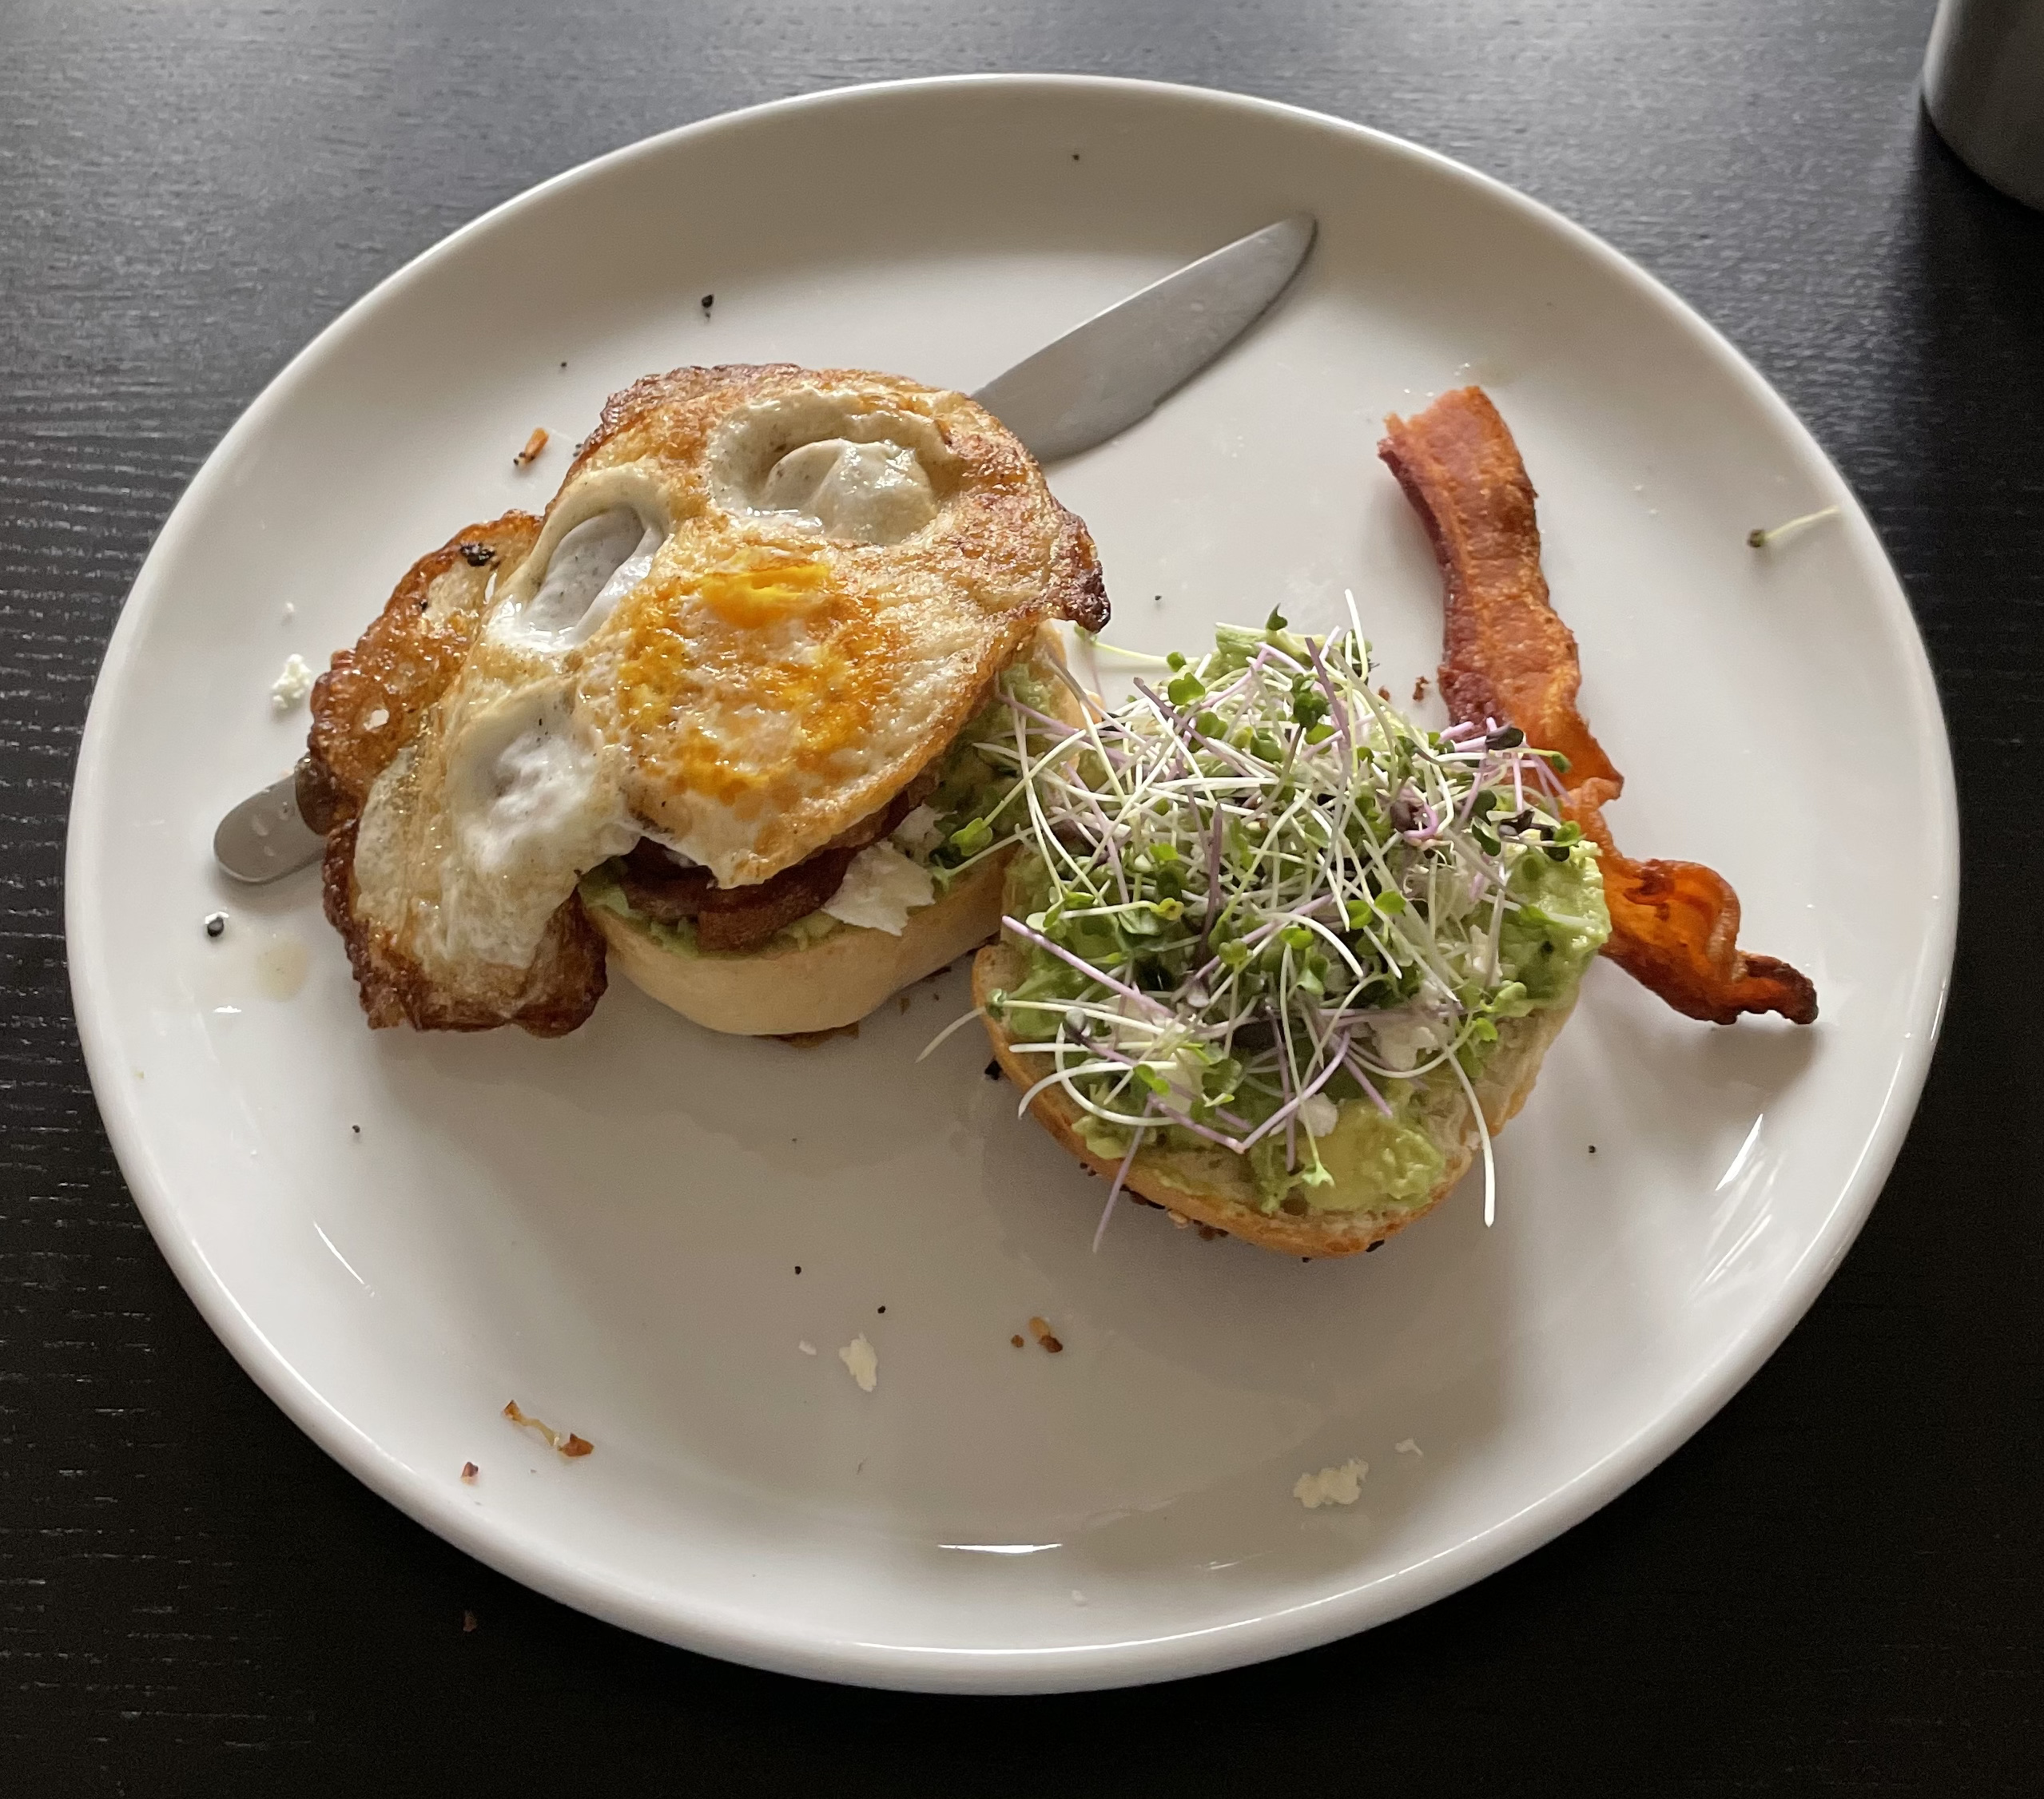
\includegraphics[width=.8\linewidth]{photos/bagels1.jpeg}  
						\end{subfigure}
						\begin{subfigure}{.5\textwidth}
								  \centering
								    % include second image
								    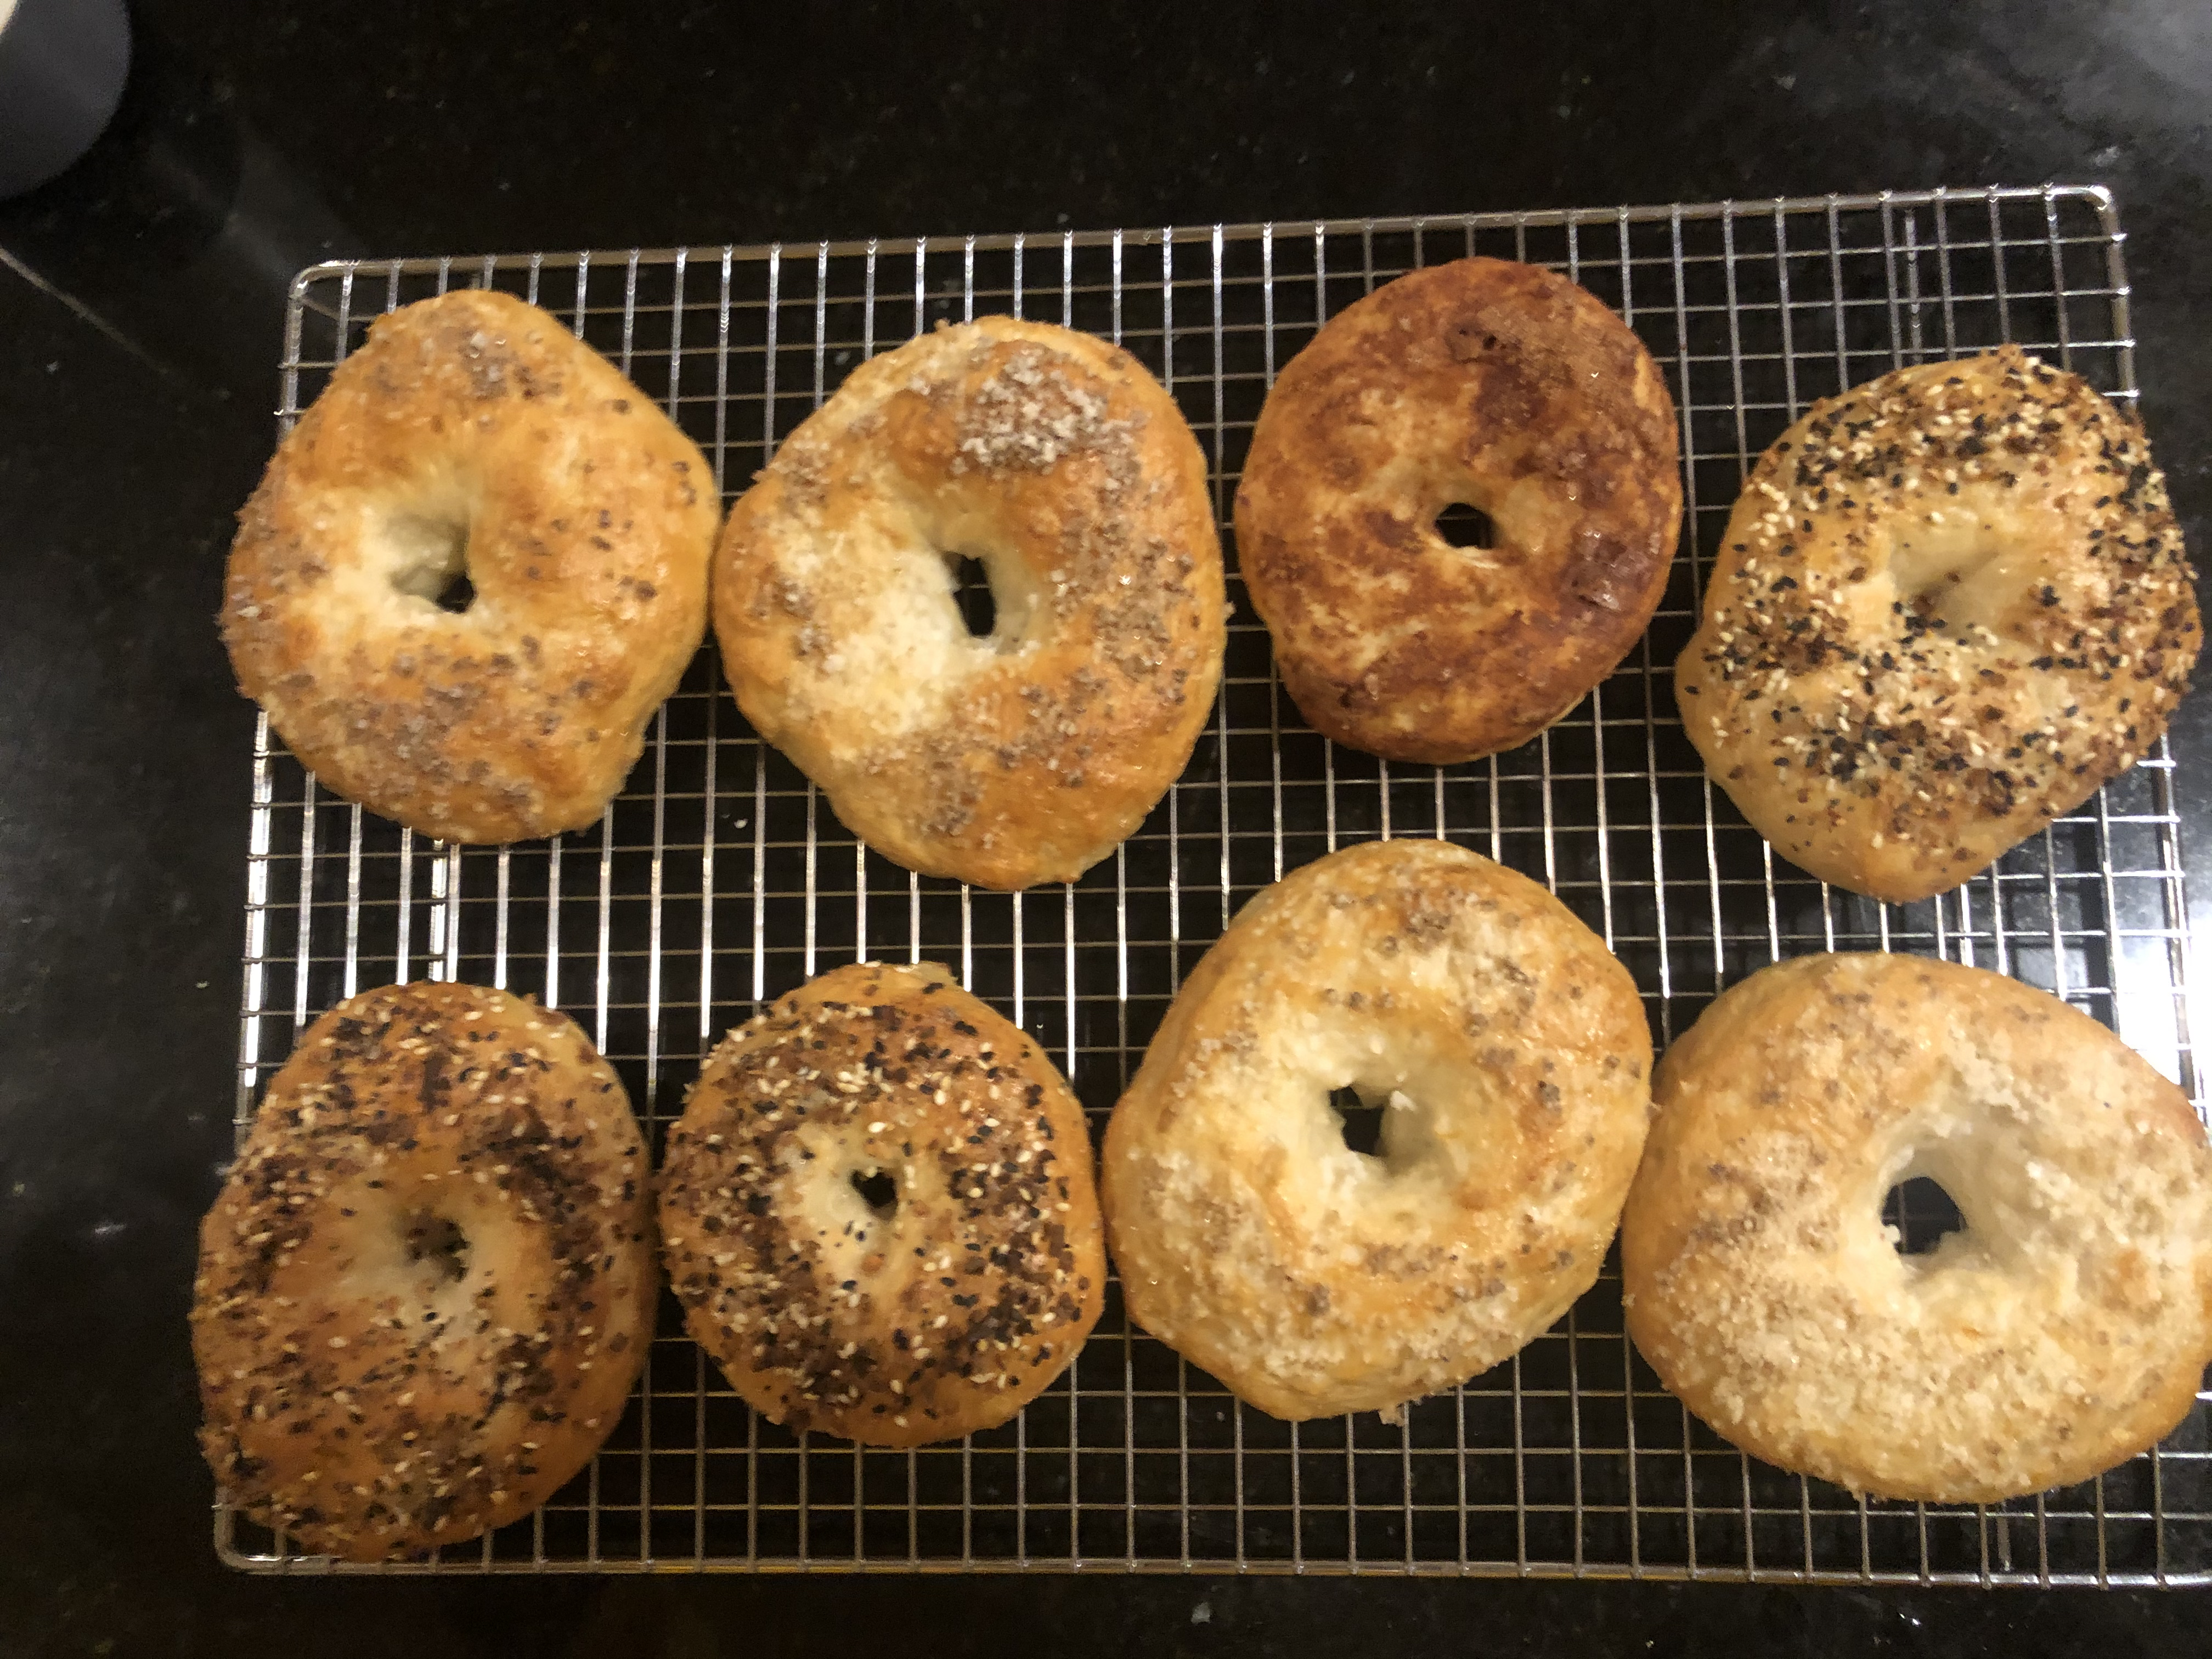
\includegraphics[width=.8\linewidth]{photos/bagels2.jpeg}  
								\end{subfigure}
						\end{figure}
		\hint{\begin{enumerate}
						\item Jalapeño cheddar bagels - grate about a cup and a half of cheddar cheese and dice 1-2 jalapenos. Add half of the cheese and the jalapeños to the dough while mixing, top the bagels with the rest of the cheese before baking.
						\item My favorite is the William-Sonoma Everything Bagel seasoning as a topping.
						\item Cinnamon-raisin bagels - Add 1 tsp vanilla extract and 3/4 cups raisins to the dough. Combine 1 tsp cinnamon and 3 tbsp granulated sugar and knead into the dough. Boil and bake as usual.
		\item other good toppings include: salt, onions, sesame seeds, or anything else you can think of!\end{enumerate}} 

						\end{recipe}
 \clearpage

\newpage
\section{Holiday favorites}
\begin{recipe}[%
preparationtime={\unit[1.5]{hours}},
portion=\portion{8-10},
source=Food\&Wine Magazine
]
{Sweet Potato Biscuits}

\ingredients[15]{
1 & medium sized sweet potato\\
\unit[1 3/4]{cups} & all-purpose flour\\
\unit[1]{tbsp} & brown sugar \\
\unit[2 1/2]{tsp} & baking powder \\
\unit[1/2]{tsp} & baking soda \\
\unit[1]{tsp} & salt \\
\unit[7]{tbsp} & cold unsalted diced butter \\
\unit[1/3]{cup} & butter milk \\
}

\preparation{
\newline
\step Preheat the oven to 375 \faren. Poke the sweet potato all over with a fork and bake for about 45 minutes, until tender. Peel and mash the potato. Set aside 3/4 cup of the mashed potato and let cool completely; reserve the rest for another use. Raise the oven temperature to 425 \faren.
\step In a food processor, pulse the flour with the brown sugar, baking powder, baking soda, and alt. Add the butter and pulse until the mixture resembles coarse meal. Add the buttermilk and the 3/4 cup mashed potato and pulse until the dough comes together.
\step Turn the dough out onto a heavily floured work surface and knead 2 or 3 times, until smooth; the dough will be soft. Roll out the dough 1/4 inch thick and cut out 8 4-inch rounds. A cup or mason jar works well here. Arrange the biscuits on a baking sheet. Bake for about 15 minutes, until golden brown. 
}
\hint{The sweet potato mashed can be made a couple days ahead and stored in the fridge. I almost always double this recipe because I have enough sweet potato}
\end{recipe}

\newpage
\begin{recipe}[
preparationtime= 1 hour 5 min,
source = Its a keeper blog]
{Thanksgiving Stuffing}
\ingredients[15]{
\unit[2]{loaves} & sandwich bread\\
\unit[12]{tbsp} & unsalted butter \\
4 & onions \\
1 & head of celery \\
\unit[2]{tbsp} & dried sage \\
\unit[1]{tbsp} & salt \\
\unit[1]{tbsp} & black pepper \\
\unit[1]{tbsp} & garlic powder \\
\unit[1]{tbsp} & onion powder\\
\unit[1/2]{cup} & vegetable broth \\
}

\preparation{
\newline
\step Cut the bread into \~ 1-inch cubes and sit out to dry over night.
\step Pre-heat oven to 350\faren. Dice the onions and celery. Melt butter in a large skillet
\step Add the onions, celery, and spices to the pan. Saute until vegetables are translucent and tender.
\step Grease a 13 x 9 baking dish. Place the bread in the dish and cover with the onion mixture and broth. Stir to combine add salt and pepper to taste. 
\step bake for about 30 minutes
}
\hint{I like to use a mixture of breads so one loaf of sourdough and one of a more fluffy bread. 2 loaves is a recommendation it depends heavily on the size of your loafs. Feel free to add more spices to taste, Rosemary and Italian seasoning are both a good addition as is some minced garlic.}
\end{recipe}


\end{document}


